\subsection{ESMF}
\par
The Earth System Modeling Framework (ESMF) is an open source project. It is build upon a scalable, flexible paradigm for building and coupling weather, climate, and other Earth science models. ESMF is based on principles of component-based software engineering \autocite{dsl:esmf-homepage}. The components within an ESMF software application usually represent large-scale physical domains such as the atmosphere, ocean, cryosphere or land surface. The framework includes regridding tools for composing complex, coupled modeling systems, and data structures and utilities for developing individual models \autocite{dsl:esmf-free_lib}.
\par
ESMF provides a complete set of Fortran interfaces and some C and C++ interfaces \autocite{dsl:esmf-tutorial1}. The view of the framework consists of two layers, an infrastructure of utilities and data structures for creating model components, and a superstructure for coupling them. User code is placed between these two layers, to make calls to the infrastructure libraries and be scheduled and synchronized by the superstructure, shown in the Figure \ref{fig:esmf_architecture} \autocite{dsl:esmf-overview}.
\begin{figure}[h]
	\centering
	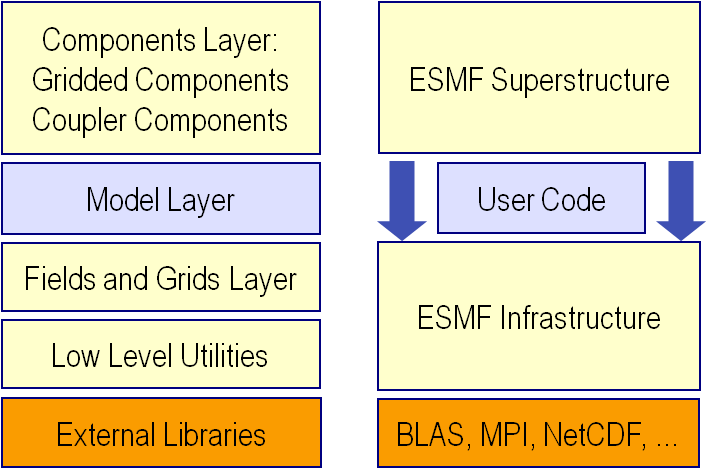
\includegraphics[width=0.7\textwidth]{pics/esmf/esmf_architecture.png}
	\caption{Schematic of the ESMF architecture \autocite{dsl:esmf-regridding} \label{fig:esmf_architecture}}	
\end{figure}
\par
Like many other frameworks, this also does not provide “instructions” that can be used immediately to develop a DSL. To create own models, knowledge in general-purpose languages is required.

\subsubsection {Properties of the modeling}
\par
The ESMF Application Programming Interface (API) is based on the object-oriented programming concept of a class. The major classes in the ESMF superstructure are Components, which typically represent large pieces of functionality such as models, model couplers, dynamics and physics packages, and States, which are the data structures used to communicate data between Components \autocite{dsl:esmf-overview}. User data is represented in the form of data objects such as grids, fields, and arrays. The user can reference a Fortran array to an ESMF array or field, or retrieve a Fortran array out of an ESMF array or field. The fields on the same grid can be collected to a bundle to optimize the performance, by sharing collective communication, IO, and regridding \autocite{dsl:esmf-tutorial2}.
\par
Data representation in index space (Arrays):
\begin{itemize}
	\item Sparse matrix multiply for regridding with user supplied interpolation weights
	\item Very general data representation, but limited interoperability since not much semantic info is encoded by the framework \autocite{dsl:esmf-enhancements}.
\end{itemize}
\par
The focus of the ESMF is to define standardized programming interfaces and to collect and provide data structures and utilities for developing model components. One disadvantage of the ESMF approach is that developers of the scientific models need to refactor their existing code to fit the interface, which is usually not easy \autocite{dsl:esmf-fortran}.
\par
Yet it is a big challenge for earth researchers to develop, maintain and share the component code due to the absence of the system software development training. Researchers have to consider about plenty of the essential framework code not related with the business logic. Furthermore, there is no unified platform which helps researchers from different institutions share component code. What’s more, at present, there is still no widely adopted Integrated Development Environments (IDE) for ESM. Therefore, developing, maintaining and sharing the component code put extra pressure on researchers, which limit the widespread use of ESMF \autocite{dsl:esmf-graphical}.
\par
To overcome these disadvantages, in the paper \autocite{dsl:esmf-graphical} an Earth System Model Component Description Language (ESMCDL) is proposed which describes not only the interface of component but also the inner behavior of the interface. At the same time, based on this language a graphical development tool is designed to help researchers encapsulate, release components and build templates which consist of these components. Results show that the tool based on the ESMCDL significantly reduces the time required to develop models.
\par
The ESMF does not provide abstractions for writing the scientific kernels, mentioned in \autocite{dsl:esmf-coupling}:
\begin{quotation}
\textit{
``The current state of the art precludes defining a DSL that meets the completeness criteria. This is based on the fact that ESMF itself does not attempt to provide abstractions for writing the scientific kernels. The highly customized nature of this kind of code is perhaps best left to a general-purpose language (GPL) where the programmer has freedom to implement the science in whatever manner seems most appropriate.''}.
\end{quotation}
\par
Due to the characteristics of the framework and the above-mentioned disadvantages, the further study of the framework is not part of this project.
















